\documentclass[11pt]{report}
\usepackage[french]{babel}
\usepackage[utf8]{inputenc}
\usepackage[T1]{fontenc}
\usepackage[top = 2cm, bottom = 2cm, left = 2cm, right = 2cm]{geometry}
\usepackage{graphicx}
\usepackage{times}
\usepackage{parskip}
\usepackage{amsfonts}
\usepackage{graphicx}
\usepackage{cprotect}
\usepackage{fancyvrb}

\title{Rapport projet IA04 ~\\ Flotte de drones en 2D}
\author
{
	Mohamed \bsc{Baaziz} ~\\ 
	Lucas \bsc{Sorin} ~\\ 
	Gustavo \bsc{Cabrera} ~\\ 
	Hachem \bsc{Benyahia}
}
\date{13 juin 2016}

\renewcommand{\thesection}{\arabic{section}}

\begin{document}

\maketitle
\renewcommand{\contentsname}{\centering Sommaire \vspace*{1cm}}
\tableofcontents

\newpage

\section{Introduction}

Dans le cadre de l'UV IA04, nous devons réaliser un SMA (\textit{Système Multi-Agents}) évolué à l'aide de la librairie JADE sous Java. L'objectif est donc donc un premier temps de trouver un fonctionnement ou un phénomène modélisable sous le paradigme multi-agents, et implémentable sous JADE, puis précisément de le coder pour ensuite pouvoir le simuler informatiquement. On peut par exemple penser à beaucoup d'exemples connus dans le domaine de l'intelligence artificielle comme le modèle proie-prédateur, l'évolution d'une population d'insectes, le comportement d'une foule, etc. 

Dans la première partie, celle qui suit cette introduction, nous allons décrire le système réel choisi à modéliser. Puis nous verrons les préférences technologiques vers lesquelles nous nous sommes tournés pour l'implémentation. Ensuite nous décrirons l'architecture du système conçu. Pour terminer, nous présenterons quelques pistes d'amélioration et enfin nous conclurons sur ce projet.

\section{Contexte}

Dans cette section, nous allons décrire le projet, en quoi il consiste, son but, son utilité, ses implications dans le monde réel, le contexte global dans lequel il se situe (en dehors de l'UV IA04) ainsi que sa faisabilité.

\subsection{Description du projet}

Comme le titre du rapport l'indique, notre choix s'est porté sur les drones, appareils sur lesquels il y a encore beaucoup à faire et dont les applications sont multiples. Ces appareils sont chers à fabriquer, et lorsque par exemple l'un d'entre eux tombe en panne, surtout s'il est isolé, on peut le considérer comme étant perdu (financièrement parlant). Le fait d'en avoir plusieurs qui se déplacent en flotte a beaucoup d'avantages. Les drones d'une flotte, avertis de la chute (sur le sol) de l'un des leurs, pourraient le rapatrier (à la base, dans un contexte militaire typiquement) et le faire réparer par des opérateurs, voire le réparer eux-mêmes (flottes autonomes).

Ceci n'est bien sûr qu'une application possible, et en pratique les flottes de drones peuvent être vues comme un réseau de drones interconnectés et communiquant entre eux afin d'atteindre un objectif donné (qui peut être se déplacer à un endroit, réguler le trafic aérien en optimisant leur déplacement dans le ciel - cas utile s'il y a plusieurs appareils volants dans l'espace en question - etc.).

On voit en quoi les drones sont adaptés au paradigme SMA, chaque drone pouvant être vu comme un agent. Bien sûr, on peut pousser le concept et donner une intelligence artificielle à chaque flotte, ainsi que permettre aux flottes de communiquer sur de très longues distances. En extrapolant, on peut même aller au-delà des drones et suggérer un système autonome d'auto-régulation de tout le trafic (routier, aérien, maritime, etc). Mais pour le projet, ce qui nous intéresse c'est uniquement la simulation d'une flotte de drones, de sa création, à éventuellement sa destruction, en passant par sa fusion avec une autre flotte.

La formation d'une flotte de drones doit être réalisée afin de répondre à un but précis ou à un ensemble d'objectifs visés. Dans notre cas, l'objectif des drones sera de traverser des portails éparpillés dans l'environnement.

Chaque portail ne pourra accepter qu'un nombre précis de drones (pas moins, ni plus). À l'entrée des drones attendus, le portail fermera ses portes et n'acceptera plus de drones.

\subsection{Contraintes}

Comme ce projet d'IA04 est limité en temps et en main-d'œuvre, il faut restreindre le cadre et spécifier les fonctionnalités que nous avons l'intention d'implémenter. En l'occurrence nous allons décrire notre cadre de conception dans la prochaine sous-partie.

\subsubsection{Modélisation} 

On suppose qu'un agent représente un drone et on se place dans un plan 2D ($xOy$). Chaque drone est assimilé à un point qui représente sa position $(x, y)$ dans le plan. La taille du point n'est pas forcément d'un pixel (on pourrait difficilement le voir dans ce cas ...). L'objectif est de faire en sorte que les agents coexistent dans un périmètre donné, leur coexistence devant amener à la formation de flottes, et à l'organisation de l'entrée des drones dans les portails (but du projet). Les coordonnées sont positives, on se place dans $\mathbb{R}^{2}_{+}$. L'espace de déplacement (l'environnement) n'est pas torique et est limité par des bornes en $x$ et $y$. L'espace est carré.

\subsubsection{Comportement des drones}

La coexistence des drones et l'organisation des voyages vers les portails sont basées sur plusieurs règles de fonctionnement : 

\begin{itemize}
\item Les drones ont tendance à s'organiser en flotte, le nombre de drones maximal dans une flotte est une constante définie au début du programme.

~\
\item Les drones sont démarrés seuls au départ et ne font pas partie d'une flotte.

~\
\item Chaque drone a un unique identifiant.

~\
\item Chaque flotte a un un maître qui guide sa flotte.

~\
\item Les flottes sont en anneau, le diamètre varie en fonction du nombre de drones dans la flotte.

~\
\item La communication des drones se fait par messages à courte portée, ce qui concrètement veut dire qu'un drone ne peut émettre qu'à un certain rayon autour de lui, et de même ne recevoir qu'à une distance inférieure ou égale à ce rayon (en pratique nous avons fait en sorte que chaque drone émette à tous les autres drones mais que les messages soient filtrés en fonction de la distance à l'émetteur).

~\
\item Lorsqu'un drone (ou une flotte) rencontre un autre drone (ou une autre flotte), une procédure est activée de manière à ce que les deux ensembles fusionnent (ou non, en fonction du nombre de drones déjà présents dans la flotte).

~\
\item Lorsqu'un drone est détruit, il est retiré de la liste des drones existants.

~\
\item La communication utilisée dans une flotte est une communication de proche en proche (communication en anneau).

~\
\item Lorsqu'un drone rencontre un portail, il enregistre en mémoire locale son nom, sa position et le nombre de drones exacte qu'il accepte.

~\
\item Lorsqu'un drone intègre un flotte, il partage avec tous les drones de sa nouvelle flotte les informations sur les portails qu'il a collecté jusque là.

~\
\item Dès que possible (portail connu disponible et nombre suffisant de drones dans sa flotte), le maître d'une flotte envoi le bon nombre de drones vers un des portails ouverts compatibles.

~\
\item Lorsqu'un drone reçoit un ordre de son maître de flotte lui demandant de voyager vers un portail, il quitte sa flotte et se dirige vers le portail. Une fois arrivé à portée du portail, il demande au portail l'autorisation d'entrer. Si il y est autorisé, il se déplace jusqu'à entrer dedans, envoi un message d'arrivée au portail, puis disparaît. Sinon, il se remet à voguer dans l'environnement en quête d'une autre flotte.
\end{itemize}

\subsubsection{Comportement des portails}

Pour organiser l'entrée des drones dans les portails, un ensemble de comportements ont du être implémentés : 

\begin{itemize}

\item Chaque portail diffuse à tous les drones à proximités son nom, sa position, et le nombre de drones qu'il souhaite faire entrer.

~\
\item Lorsqu'un drone maître demande d'envoyer un ensemble de drones, le portail lui réserve ses places si aucun autre maître ne l'a fait avant lui. Le portail joint à son message d'acceptation un mot de passe qui servira à l'authentification des futurs drones envoyés.

~\
\item Lorsqu'un drone demande d'entrer, le portail vérifie son mot de passe contenu dans son message, puis en fonction de cette vérification, envoie un message d'autorisation ou de refus.

~\
\item Un portail ferme ses portes lorsqu'il a reçus tous les messages d'arrivée des drones attendus.
\end{itemize}

\section{Choix technologiques}

Pour concevoir ce système, nous avons fait quelques choix en terme de technologies. Bien sûr, la contrainte du projet est la librairie JADE. Mais il y a également d'autres points à préciser.

\subsection{Interface graphique}

Pour afficher les drones, nous avons utilisé une interface graphique. Cette partie était facultative, mais il aurait été difficile de visualiser leur déplacement dans une console, et donc une GUI (\textit{Graphical User Interface}) semblait particulièrement adaptée à ce cas de figure.

Le rendu visuel est quelque chose comme ceci par exemple (captures faites en cours de développement, on ne voit pas de flottes en anneau, mais certains drones se sont rejoints et se suivent comme on peut le voir de la première capture à la deuxième) :

Un drone est représenté par un carré blanc, tandis qu'un portail est représenté par un carré de couleur.

\begin{figure}[h]
\centering
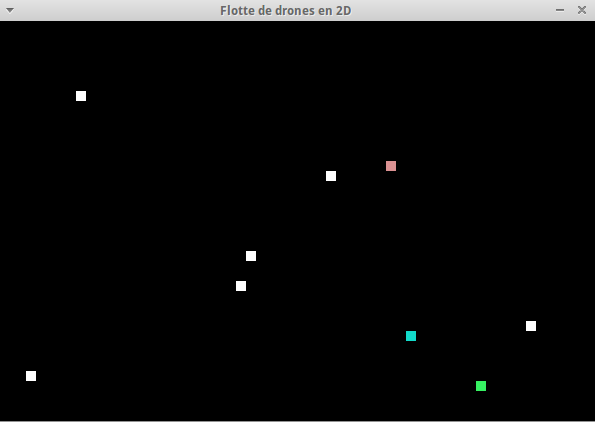
\includegraphics[scale = 0.9]{img/flotte-3.png}
\caption{5 drones sont en train de déplacer (librairie libsdl)}
\end{figure}

\begin{figure}
\centering
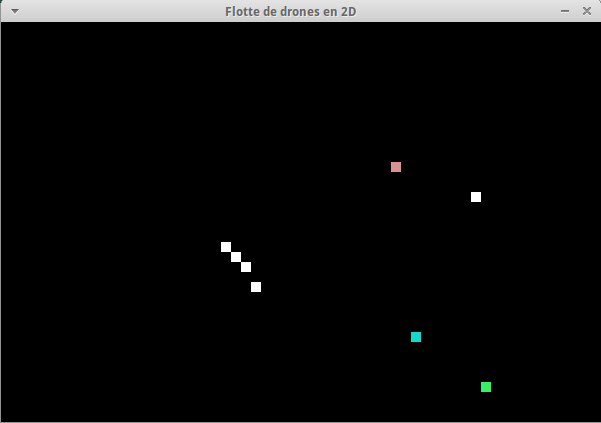
\includegraphics[scale = 0.9]{img/flotte-4.png}
\caption{Les drones se déplacent encore (librairie libsdl)}
\end{figure}

\clearpage

\subsubsection{sdljava (ou libsdl)}

Pour cette interface graphique, nous avons utilisé la librairie \textbf{sdljava}, qui est un \textit{binding} de la librairie \textbf{SDL} du langage C pour le langage Java. Cette librairie est particulièrement adaptée grâce à sa légèreté (une classe suffit à générer la fenêtre graphique).

\subsection{Communication}

La communication des agents Jade (drones et portails) utilisés dans ce projet se fait en JSON.

\section{Architecture}

Nous allons à présent décrire l'architecture du projet.

L'architecture se divise en quatre parties : les drones qui évoluent dans l'environnement 2D, les objets qui se trouvent sur le terrain (partie qui n'a pas été implémentée), les portails et l'interface graphique qui va représenter tout cela sur l'écran. Ces trois parties sont plus ou moins indépendantes. À cela s'ajoutent certaines classes utilitaires et fichiers de constantes. 

Nous n'allons dans ce rapport décrire que ces quatre segments, car les autres éléments sont moins pertinents pour l'objet de ce rapport, l'objectif de cette partie étant surtout d'avoir une vue globale du fonctionnement du programme.

\subsection{L'agent \protect\Verb+Drone+}

\subsubsection{Description}

La classe \verb|Drone| est la principale classe du projet. En termes de cardinalité, le nombre d'instances de cette classe peut varier de $1$ à $n$.

\subsubsection{Attributs}

Quelques attributs en vrac de la classe \verb|Drone| :

\begin{enumerate}
\item La position actuelle du drone dans le plan $p = (x, y)$ qui est représentée la classe \verb|Position|, qui définit un certain nombre de méthodes (par exemple renvoyer la distance entre deux points du plan).

\item Un identifiant unique.

\item Un état qui indique sa disponibilité (s'il est dans une flotte ou seul par exemple, s'il est actuellement en train de s'intégrer à une flotte existante, s'il est mort ou en voyage vers un portail etc.).

\item La position objectif du drone (le drone a un objectif par défaut qu'il veut atteindre quand il n'est pas sous la tutelle d'une flotte).

\item Le maître de sa flotte, s'il appartient à une flotte.

\item Son rang dans la flotte et le voisin auquel il doit envoyer un message (anneau unidirectionnel), s'il appartient à une flotte.

\item Les informations des portails rencontrés.

\item Le portail choisi comme destination (initialement vide).

\item Le mot de passe attribué (initialement vide), qui servira à l'authentification du drone auprès du portail.
\end{enumerate}

\subsubsection{Behaviours} 

Le drone réagit à son environnement de plusieurs manières, dépendamment des stimuli qui lui parviennent. 

Voici quelques behaviours de la classe \verb|Drone| :

\begin{enumerate}
\item \textbf{RespondToDisplay} : Un behaviour cyclique qui renvoie la position de l'agent à l'agent \verb|Display| (que nous allons introduire plus loin) quand il le lui demande.

\item Un behaviour qui envoie spontanément un message à l'agent \verb|Display| lors de la mort de l'agent (l'agent \verb|Display| doit dans ce cas supprimer le drone de la liste des drones et mettre à jour l'affichage). (ce comportement est inclus dans \textbf{ReceiveEnvironment})

\item \textbf{ReceiveEnvironment} : Un behaviour qui réagit aux messages provenant de d'autres éléments de la classe \verb|Drone|.

\item \textbf{EmitEnvironment} : Un behaviour de type Ticker qui envoie périodiquement des messages dans l'environnement immédiat de l'agent (il se contente d'émettre aux autres agents, la réception du message se fait par une fonction de filtration sur l'attribut représentant la position).

\item Un behaviour qui réagit aux messages provenant des objets (dans cette modélisation, les objets sont des ensembles de points fixes dont les points périphériques envoient périodiquement des messages aux drones). (ce behaviour n'a pas été implémenté au regard du manque de temps pour ce projet)

\item \textbf{Movement} : Un behaviour de type Ticker qui à chaque itération réalise le déplacement approprié. Si le drone est tout seul, alors il suis une position objectif aléatoirement choisie. S'il a déjà atteint cette position, il en choisi une autre. Si le drone est en flotte, alors il suis le déplacement de son drone maître. Lorsqu'il est en état de voyage (vers son portail), il se déplace vers le portail. S'il est en attente d'une réponse de la part du portail, alors il reste immobile.

\item \textbf{ReceivePortalsInfos} : Un behaviour qui écoute la diffusion des portails, et enregistre en mémoire les informations broadcastées.

\item \textbf{ReceiveMasterOrder} : Un behaviour qui écoute les ordres venant de son maître de flotte (ex. ordre de voyage vers un portail).

\item \textbf{PortalAccept/PortalRefuse} : Deux behaviours qui écoutent les réponses venant du portail que le drone souhaite traverser. Accept $\rightarrow$ entre dans le portail, Refuse $\rightarrow$ reprend son comportement initiale, à la recherche d'une nouvelle flotte.

\item \textbf{InitiateLandingRequest} : Un behaviour de type oneshote qui, lorsqu'il est instancié, se charge de proposer (message de type PROPOSE) un envoi de drone au portail choisi (le nom du portail est donné en argument lors de son instanciation).
\end{enumerate}

\subsection{L'agent \protect\Verb+Display+}

\subsubsection{Description}

La classe \verb|Display| est une classe indépendante de la classe \verb|Drone|. Son rôle est de rapatrier les positions des drones et de les afficher sur une interface graphique. L'implémentation de cette classe passe donc par l'utilisation de sdljava. 

En termes de cardinalité, le nombre d'instances de cette classe est exactement de $1$. C'est la première classe créée lors du lancement du programme, et elle crée les autres objets dès son démarrage. Elle initialise les position des drones (qui peuvent éventuellement être passées en paramètres dans une implémentation plus poussée) et des objets.

\subsubsection{Attributs}

Quelques attributs en vrac de la classe \verb|Display| :

\begin{enumerate}
\item Un tableau dynamique (du fait de la suppression possible de drones au cours de l'évolution de la simulation) recensant les drones existants et leurs positions.

\item Le nombre de drones existants.

\item Un tableau dynamique recensant les objets sur le terrain (non implémenté).

\item Le nombre d'objets existants (non implémenté).

\end{enumerate}

\subsubsection{Behaviours}

Voici quelques behaviours de la classe \verb|Display| :

\begin{enumerate}
\item \textbf{RetrievePositions} : Un behaviour de type Ticker qui envoie périodiquement à tous les agents \verb|Drone| une demande de leur position. Il met à jour le tableau de positions.

\item \textbf{DeathDetector} : Un behaviour cyclique qui écoute les signaux de mort de la part d'une drone et le supprimer de sa liste de drones.

\item Un behaviour qui répond un signal d'arrêt en provenance de la console, il supprimera tous les drones et objets et terminera l'exécution (cela n'a pas été implémenté).
\end{enumerate}

\subsection{L'agent \protect\Verb+Object+ (non implémenté)}
\subsubsection{Description}

La classe \verb|Object| n'a pas été implémentée. Elle représente les objets qui se trouvent sur le terrain. Les objets sont des polygones. Un objet est un ensemble de points dont les points frontaliers sont ceux qui émettent des messages (il est important de rappeler que les points ne sont pas des pixels, mais des surfaces carrées d'une certaine dimension).

\subsubsection{Attributs}

Quelques attributs en vrac de la classe \verb|Object| :

\begin{enumerate}
\item Un tableau de points représentant la totalité des points qui le composent.

\item Un identifiant unique.
\end{enumerate}

\subsubsection{Behaviours}

Voici quelques behaviours de la classe \verb|Object| :

\begin{enumerate}
\item Un behaviour qui émet constamment des messages (destinés aux agents) dans les environs de l'objet. Seuls les points frontaliers doivent émettre des messages.

\item Un behaviour qui renvoie l'ensemble des points le constituant à l'agent \verb|Display| lorsqu'il le lui demande.
\end{enumerate}

\subsection{L'agent \protect\Verb+Portal+}

\subsubsection{Description}

La classe \verb|Portal| est l'une des classe les plus importantes de notre système multi-agents (avec \verb|Drone|). Son existence donne un objectif percevable à notre simulation. Le rôle d'un agent \verb|Portal| est d’accueillir un nombre de drones compris (déterminé lors de sa création par l'agent display).

\subsubsection{Attributs}
Voici les principaux attributs de la classe \verb|Portal| :

\begin{enumerate}
\item Un identifiant unique.

\item Un entier désignant le nombre de drones acceptés.

\item La position du portail.

\item Un booléen qui désigne la disponibilité du portail (devient faux après qu'un drones maître ai réservé ses places).

\item Un booléen qui permet de savoir si le portail et ouvert ou fermé (se ferme lorsque tous les drones attendus sont entrés).

\item Le mot de passe communiqué au dernier drone maître dont la proposition a été acceptée. Il est réutilisé pour vérifier l'authenticité des drones entrants.

\item Un tableau stockant les identifiants des drones attendant à l'entrée du portail, en attente d'une autorisation. Ceci permet au portail d'attendre pendant une durée déterminée les drones retardataires. Une fois ce temps écoulé, si tous les drones attendus en sont pas arrivés, les drones arrivés et en attentes seront rejetés.
\end{enumerate}

\subsubsection{Behaviours}

Voici les principaux behaviours de l'agent \verb|Portal| :

\begin{enumerate}
\item PlacesBroadcast : ticker behaviour qui périodiquement transmet à tous les drones à proximité (messages filtrés selon la distance) le nom du portail (Portal + identifiant), sa position et le nombre de drones qu'il accepte.

\item receiveLandingRequest : behaviour cyclique qui écoute les demandes des drones maître. Ces drones maîtres demandes s'ils peuvent envoyer leur drones (messages de type \verb|PROPOSE|). Le portail répond par la suite par une acceptation (\verb|ACCEPT_PROPOSAL|) ou par refus (\verb|REJECT_PROPOSAL|) en fonction de sa disponibilité.

\item ResetPassword : behaviour de type waker behaviour qui s’exécute après une certaine durée de temps et qui réinitialise le mot de passe si tous les drones attendus ne sont pas encore arrivés.

\item receiveDrones : behaviour de type cyclique qui écoute les demandes d'entrées des drones (une fois qu'ils sont arrivés à proximité). Le portail vérifie s'ils ont le bon mot de passe (contenu dans le message envoyé par les drones). Si le mot de passe est bon, alors il ajoute ce drone dans la liste des drones en attente d'une réponse. Dès que la liste des drones en attente atteint le nombre de drones attendus, le portail envoie à tous ces drones une autorisation d'entrer.
\end{enumerate}

\subsection{La classe \protect\Verb+GUI+}
\subsubsection{Description}

La classe \verb|GUI| est la classe représentant l'interface graphique. Son intégration dans le SMA décrit précédemment a été particulièrement épineuse par construction de son fonctionnement. En effet, comme cette classe contient un \textit{while} qui s'exécute en permanence dans l'attente d’événements provenant de la GUI, son instanciation bloque le code. De telle sorte que pour qu'elle libère la JVM et que les autres agents puissent s'exécuter également, il a fallu en faire un agent. De manière à ce qu'elle se \textit{détache} de la classe appelante (celle qui l'instancie). Cependant, comme son constructeur est toujours basé sur un \textit{while}, ce n'est qu'un agent sur la forme, et donc elle ne possède pas de behaviours.

Pour rafraîchir l'interface, elle appelle périodiquement une méthode qui dispose d'une \textit{référence} sur l'agent \verb|Display| afin d'acquérir des informations sur l'état actuel des drones. De tel sorte que bien que cette classe soit un agent, \textbf{elle ne communique pas par messages}.

\subsubsection{Attributs}

Quelques attributs en vrac de la classe \verb|GUI| :

\begin{enumerate}
\item Une référence sur l'agent \verb|Display|.

\item Un tableau de surfaces (concept de la librairie sdljava) représentant chaque drone et sa couleur.

\item Une référence sur l'écran actuel (la GUI), ce qui est également lié à sdljava.

\item Un tableau recensant les drones de l'itération précédente. Il permet de détecter les disparition de drones (morts ou buts atteints) et d'adapter l'interface graphique en conséquence.
\end{enumerate}

\section{Pistes d'amélioration}

Pour améliorer notre projet de simulation de flottes de drones, nous avons pensé à 3 fonctionnalités importantes que nous n'avons pas pu implémenter par manque de temps :

\begin{enumerate}
\item L'ajout d'agents Objets qui façonneraient l'environnement à la manière d'obstacles et de décors. Leur collision entraînerait la mort du drone.
\item L'ajout de configurations de flottes plus développés. En effet nous aurions par exemple souhaité que les drones puissent garder une configuration graphique en anneau.
\item L'ajout d'un calcul de trajectoire plus intelligent. En effet, en raison de la génération aléatoire des positions objectifs, il peut arriver que les maîtres de flotte choisissent une direction qui les fera rentrer en collision avec les drones qui le suivent. Or ceci pourrait être évité en implémentant un algorithme de choix de trajectoire plus intelligent qui prendrait en compte les positions des objets environnants.
\end{enumerate}

\newpage

\section{Conclusion}

Nous avons pu au travers de ce projet mettre en pratique les enseignements en systèmes multi-agents acquis tout au long du semestre pour implémenter un concept dont les applications concrètes ne manquent pas. Nous avons ainsi expérimenté les avantages et inconvénients de la conception multi-agents. En effet, des efforts ont du être faits pour sérialiser des messages complexes, mais aussi pour adapter l'utilisation d'une interface graphique aux systèmes multi-agents. Cependant, nous avons pu bénéficier de la simplicité architecturale qu'engendre l'utilisation du paradigme multi-agents. En effet, la répartitions des tâches en agents et behaviours a permis une conception claire, et naturelle. D'autant plus que dans notre cas, la plupart des agents bénéficiaient d'un sens physique mentalement concevable.

\end{document}